% !TeX spellcheck = nl_NL
\chapter{Optimalisatie sturing}
In dit hoofdstuk worden de voorgestelde optimalisaties aan het platform gedocumenteerd. De belangrijkste optimalisatie komt eerst, het verleggen van de rekenkracht naar de PC. Daarna worden de aanpassingen binnen het optical flow algoritme belicht. Vervolgens komen de PID-regelaars voor zowel hoogte als positie aan bod. Tenslotte wordt de nieuwe APM logica beschreven.

\section{Beperkte rekenkracht van Raspberry Pi omzeilen}
Om de beperkte rekenkracht van de Raspberry Pi te omzeilen, wordt voorgesteld een computer te gebruiken voor het berekenen van optical flow. Een standaard laptop zou rekenkracht genoeg moeten bieden om de resolutie van de camerabeelden waarmee optical flow berekend wordt omhoog te krijgen zonder verlies aan frame rate. De oorspronkelijke frame rate bedroeg \SI{20}{\Hz}.

\npar Dit idee kan verantwoord worden met behulp van enkele kleine berekeningen. Stel dat de verbinding tussen RPi en PC ongeveer 4 MB/s bedraagt. Dit is de gemiddelde snelheid van de WiFi-dongle die gebruikt zal worden. Er moet een afbeelding met grijswaarden van $b$ bij $l$ pixels verstuurd worden. Men kan ervan uitgaan dat 1 grijze pixel uit 8 bits of 1 byte bestaat. De grootte van 1 frame wordt dan gegeven door \eqref{eq:grootte1grame}. Stel dat de tijd nodig voor het zenden van een frame en het berekenen van optical flow vectoren kan verwaarloosd worden. Dan wordt het maximaal haalbaar aantal frames per seconde gegeven door \eqref{eq:FPSmax}.
\begin{equation}
Grootte_{1frame} = b \cdot l \cdot \SI{1}{\byte} 
\label{eq:grootte1grame}
\end{equation}
\begin{equation}
FPS_{max} = \frac{\SI{4}{\mega\byte}/s}{Grootte_{1frame}}
\label{eq:FPSmax}
\end{equation}

\npar Aan de hand van de berekening in de vorige paragraaf wordt nagegaan wat de hoogste resolutie is die een frame rate hoger dan \SI{20}{\Hz} oplevert. De resultaten staan opgelijst in tabel \ref{table:resolutieTheorie}. Er kan besloten worden dat de maximale resolutie 320 bij 240 zal bedragen. Er moet wel opgemerkt worden dat compressie er misschien voor kan zorgen dat voor 640 bij 480 pixels toch nog de kaap van \SI{20}{\Hz} bereikt wordt. Meer hierover later in deze sectie. Samengevat, het zou mogelijk moeten zijn de optical flow bereking te versnellen en preciezer te maken door de rekenkracht te verleggen naar de PC.

\begin{longtable}{lc}
		\caption{Het maximaal haalbaar aantal frames per seconde gegeven de resolutie wanneer optical flow op de PC wordt berekend.}\label{table:resolutieTheorie}
		\cr 
		\hline
		Resolutie & $FPS_{max}$\\
		\hline
		160x120 & \SI{184}{\Hz}\\
		320x240 & \SI{55.6}{\Hz}\\
		640x480 & \SI{13.6}{\Hz}\\
		\hline
\end{longtable}

\npar Ten slotte kan de lezer zich nog afvragen of de voorgestelde aanpak dan nog steeds tot de in \ref{sec:lcsturing} beschreven lokale sturing behoort. In principe niet. Het is wel zo dat ervan uitgegaan wordt dat op termijn de rekenkracht van de hardware op het platform hoog genoeg zal zijn om alle berekeningen op zich te nemen.

\subsection{Optical flow op PC}
De gewenste nieuwe architectuur van het platform wordt schematisch weergegeven in figuur \ref{fig:RPIloop2}. De belangrijkste keuzes tijdens de implementatie van deze architectuur worden hierna overlopen.

%figuur nieuwe architectuur
\begin{figure}[ht]
	\centering
	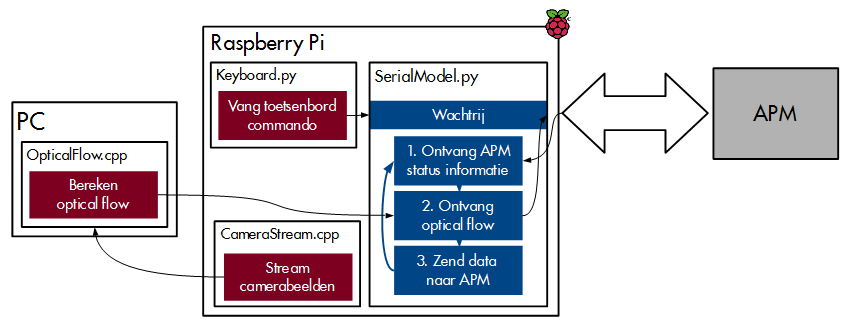
\includegraphics[width=0.9\linewidth]{RPIloop2}
	\caption{Schematische voorstelling van de nieuwe architectuur van het platform.}
	\label{fig:RPIloop2}
\end{figure}

\npar Het optical flow algoritme wordt uit de OpenCV bibliotheek ge\"importeerd \cite{url:opencv}. Zoals reeds eerder vermeld is optical flow tijdkritisch. Alle optical flow gerelateerde code wordt steeds in C ge\"implementeerd. C is dan ook de programmeertaal naar keuze bij tijdkritische applicaties \cite{paper:cpythonbenchmark}\cite{paper:cpythonbenchmark2}.

\subsubsection{CameraStream.cpp}
Aan de kant van RPi draait het programma $CameraStream.cpp$. Dit C programma wordt gebruikt om camerabeelden van de RPi naar de PC te versturen. CameraStream.cpp verstuurt de afmetingen van een frame naar de PC om vervolgens ieder nieuw frame onmiddellijk door te sturen. Alle data wordt verstuurd gebruik makend van een \textit{blocking send}. Zo wordt verzekerd dat CameraStream.cpp wacht om een nieuw frame te versturen wanneer het vorige nog niet volledig is ontvangen.

\subsubsection{OpticalFlow.cpp}
Aan de PC-kant draait $OpticalFlow.cpp$. Dit C programma staat in voor de berekening van optical flow. Via een \textit{blocking receive} worden eerst de afmetingen van ieder frame ontvangen. Ook via een \textit{blocking receive} wordt ieder nieuw frame ontvangen. De optical flow vectoren die hieruit resulteren worden dan met een \textit{non-blocking send} naar het serieel model op de RPi gestuurd. Op die manier kan OpticalFlow.cpp onmiddellijk het volgende frame ontvangen, zonder te moeten wachten tot het serieel model de flow vectoren heeft ontvangen.

\subsubsection{ZeroMQ}
Om communicatie tussen een C programma op de RPi en een C programma op de PC tot stand te brengen wordt gebruik gemaakt van de ZeroMQ bibliotheek \cite{url:ZeroMQ}. ZeroMQ werd gekozen omdat het een heel eenvoudige interface heeft. Bovendien is het ook makkelijk om berichten tussen Python en C programma's uit te wisselen. Deze eigenschap kan gebruikt worden om de berekende optical flow vectoren te sturen naar het serieel model op de RPi. Als communicatie protocol wordt TCP (Transmission Control Protocol) gekozen. TCP heeft een maximale pakketgrootte die kleiner is dan de grote van 1 frame. Om een camerabeeld van de RPi naar de PC te versturen moet het eerst worden onderverdeeld in een aantal deelpakketten. TCP is een \textit{best effort} protocol. Er wordt gebruik gemaakt van retransmissie indien pakketten verloren gaan. Het is belangrijk dat alle delen van een camerabeeld  worden ontvangen, anders kan het optical flow algoritme geen nuttige data opleveren.
% referentie naar ZeroMQ

\subsection{Compressie}
Het zou na\"ief zijn er vanuit te gaan dat het doorsturen van ruwe data van RPi naar PC de best mogelijke oplossing is. Compressie kan er in veel gevallen voor zorgen dat data sneller verstuurd wordt. Er moet gezocht worden naar een methode die weinig rekenkracht vergt aan de encoder kant, want die is nu eenmaal beperkt bij de RPi. Met deze voorwaarde in gedachten, wordt eerst gekozen voor LZ4. LZ4 behoort bij de beste compressie bibliotheken op vlak van encodeer- en decodeersnelheid \cite{url:quicklzbench}. Helaas is het niet gelukt om LZ4 werkend te krijgen op de RPi. Daarom wordt uiteindelijk gekozen voor QuickLZ \cite{url:quicklz}, ook \'e\'en van de betere compressie bibliotheken als het op snelheid aankomt \cite{url:quicklzbench}. QuickLZ werkt onmiddellijk zonder problemen.
% referentie naar quicklz vs others.
% referentie naar quicklz site

\subsection{Resultaat} \label{sec:resultaatVerleggen}
De snelheid van het optical flow algoritme wordt berekend aan de PC-kant door de tijd tussen twee opeenvolgende frames te meten. Dezelfde resoluties als in tabel \ref{table:resolutieTheorie} worden bekeken. Het gemiddeld aantal frames per seconde voor zowel met en zonder compressie wordt in tabel \ref{table:resolutieRPI} weergegeven.

% tabel met RPI1 no compr, compr FAST detector!!
\begin{table}
	\centering
	\caption{Het aantal frames per seconde gegeven de resolutie wanneer optical flow op de PC wordt berekend met Raspberry Pi 1 en Raspberry Pi 2}\label{table:resolutieRPI}
	\begin{tabular}{lcccc}
		\cr
		\hline
		& \multicolumn{2}{c}{Raspberry Pi 1} & \multicolumn{2}{c}{Raspberry Pi 2}\\
		\hline
		Resolutie & $FPS_{zonder\ compresie}$ & $FPS_{met\ compressie}$ & $FPS_{zonder\ compresie}$ & $FPS_{met\ compressie}$\\
		\hline
		160x120 & \SI{30.1}{\Hz} & \SI{29.9}{\Hz} & \SI{30.1}{\Hz} & \SI{30.1}{\Hz}\\
		320x240 & \SI{19.7}{\Hz} & \SI{15.5}{\Hz} & \SI{29.5}{\Hz} & \SI{29.7}{\Hz}\\
		640x480 & \SI{6.5}{\Hz} & \SI{5.1}{\Hz} & \SI{17.8}{\Hz} & \SI{12.6}{\Hz}\\
		\hline
	\end{tabular}
\end{table}

\npar In \ref{sec:quadcoptersturing} werd reeds aangehaald dat naar het einde van deze thesis toe, de RPi\,2 in gebruik genomen wordt. Het leek dan ook noodzakelijk om bovenstaande tests uit te voeren voeren voor de nieuwe versie van de RPi. De resultaten zijn ook opgelijst in tabel \ref{table:resolutieRPI}.

\npar Er kan besloten worden dat door het verleggen van het optical flow algoritme naar de PC, de resolutie verhoogd kan worden naar 320 bij 240 pixels om een zelfde frame rate te halen.  Voor de RPi\,1 wordt zonder compressie een frame rate van \SI{20}{\Hz} gehaald. De RPi\,2 haalt zelfs 30 frames per seconde, dit is de maximale snelheid waarmee de camera beelden kan registreren. Opmerkelijk is dat het gebruik van compressie niet zorgt voor betere prestaties. Zelfs een snelle compressie methode als QuickLZ blijkt te traag te werken op de RPi, waardoor compressie het aantal frames per seconde verlaagt in plaats van het te verhogen.

\npar Optical flow op de PC uitvoeren brengt wel \'e\'en groot nadeel met zich mee. Door de PC erin te betrekken wordt een extra vertraging toegevoegd. Dit wil zeggen dat de correcte optical flow data pas later beschikbaar zal zijn. Deze vertraging wordt gemeten in de APM en bedraagt drie tijdstappen en dus \'e\'en tijdstap meer dan voorheen. Waarschijnlijk zal dit geen probleem opleveren bij driftcompensatie.

\section{Optical Flow} \label{sec:OptFlowopt}
In de thesis van W. De Gucht werd een onderzoek gedaan naar de beste feature detector om optical flow mee te combineren. Good Features to Track (GFTT) \cite{paper:GFTT} bleek het best te presteren. De RPi is echter niet krachtig genoeg om deze detector te gebruiken voor een realtime toepassing. Daarom werd de Features from Accelerated Segment Test (FAST) \cite{paper:FAST} detector gebruikt. Gezien rekenkracht nu geen probleem meer mag zijn, wordt onderzocht of GFTT wel degelijk een betere prestatie oplevert. Eerst wordt de werking van beide detectors kort uitgelegd en vervolgens wordt hun prestatie vergeleken.

\subsection{FAST detector} \label{sec:FAST}
De FAST feature detector wordt beschreven door E. Rosten et al. in ``Machine learning for high-speed corner detection"\cite{paper:FAST}. Er wordt gebruik gemaakt van een getrainde decisieboom om te bepalen of een pixel een goeie feature is of niet.

\npar FAST heeft zijn naam niet gestolen. Deze detector werkt erg snel omdat geen zware berekeningen moeten gebeuren. Er moeten enkel een aantal geneste \textit{if-lussen} doorlopen worden.

\npar De detector heeft wel \'e\'en groot nadeel, FAST is erg gevoelig voor ruis. In de praktijk houdt dit in dat wanneer de quadcopter snel beweegt en de camerabeelden wazig worden, de detector veel minder goeie features vindt. Optical flow data is dan ook niet meer even betrouwbaar, wat belangrijke gevolgen kan hebben voor driftcompensatie.

\subsection{GFTT detector}
De GFTT feature detector wordt beschreven door J. Shi et al. in ``Good Features to Track"\cite{paper:GFTT}. Deze detector gaat features selecteren door ze te evalueren over meerdere frames. Er wordt een maat van ongelijkheid bijgehouden voor elke feature, die wordt ge\"updatet bij ieder nieuw frame. Wanneer een feature te veel begint te verschillen van hoe het er origineel uit zag, wordt de feature verwijderd uit de selectie. De resulterende feature verzameling is hierdoor optimaal voor het huidige frame. GFTT heeft wel als nadeel dat het veel meer rekenkracht eist dan de FAST detector.

\subsection{Resultaat}
Om de prestatie van beide detectors te vergelijken, wordt een zekere afstand afgelegd met de quadcopter in de hand. Er wordt afwisselend snel en traag gelopen, op die manier zullen zowel wazige als scherpe beelden geregistreerd worden. Alle camerabeelden worden opgeslagen en optical flow wordt berekend met beide detectors. De resulterende optical flow vectoren kunnen nu vergeleken worden om te zien welke detector het best presteert.

% figuur met scherpe beelden
\begin{figure}
\begin{center}

\subfigure[Frame 1]{\includegraphics[width=0.45\linewidth]{TestScherp/frame1}}
\hspace{0.01\linewidth}
\subfigure[Frame 2]{\includegraphics[width=0.45\linewidth]{TestScherp/frame2}}
\end{center}

\begin{center}
\subfigure[FAST]{\includegraphics[width=0.45\linewidth]{TestScherp/FAST}}
\hspace{0.01\linewidth}
\subfigure[GFTT]{\includegraphics[width=0.45\linewidth]{TestScherp/GFTT}}
\end{center}
\centering
\caption{Flow vectoren voor optical flow in combinatie met FAST en GFTT voor scherpe beelden. Bij scherpe beelden vindt de GFTT detector(d) meer features dan de FAST detector(c). De features gevonden door beide detectors zijn van goeie kwaliteit.}\label{fig:scherp}
\end{figure}


\npar In figuur \ref{fig:scherp}(a) en \ref{fig:scherp}(b) zijn twee scherpe beelden te zien. De resulterende optical flow vectoren voor respectievelijk de FAST- en GFTT detector worden weergegeven in \ref{fig:scherp}(c) en \ref{fig:scherp}(d). Er kan afgeleid worden dat voor scherpe beelden, GFTT meer features vindt dan FAST.
% aanvullen met bevindingen

% figuur met wazige beelden
\begin{figure}
\begin{center}
\subfigure[Frame 1]{\includegraphics[width=0.45\linewidth]{TestWazig/frame1}}
\hspace{0.01\linewidth}
\subfigure[Frame 2]{\includegraphics[width=0.45\linewidth]{TestWazig/frame2}}
\end{center}

\begin{center}
\subfigure[FAST]{\includegraphics[width=0.45\linewidth]{TestWazig/FAST}}
\hspace{0.01\linewidth}
\subfigure[GFTT]{\includegraphics[width=0.45\linewidth]{TestWazig/GFTT}}
\end{center}
\centering
\caption{Flow vectoren voor optical flow in combinatie met FAST en GFTT voor wazige beelden. De GFTT detector(d) vindt duidelijk veel meer features dan de FAST detector(c) wanneer het beeld wazig wordt. Bovendien zijn de features die de FAST detector vindt niet allemaal van goeie kwaliteit, terwijl dit wel het geval is bij de GFTT detector.}\label{fig:wazig}
\end{figure}

\npar In figuur \ref{fig:wazig}(a) en \ref{fig:wazig}(b) zijn twee wazige beelden te zien. De beelden zijn wazig door de snelheid waarmee de quadcopter beweegt. De resulterende optical flow vectoren voor respectievelijk de FAST- en GFTT detector worden weergegeven in \ref{fig:wazig}(c) en \ref{fig:wazig}(d). GFTT bewijst zijn meerwaarde vooral bij wazige beelden. FAST vindt erg weinig flow vectoren, en enkele ervan zijn zijn zelfs niet correct. GFTT vindt een stuk meer flow vectoren die allemaal wel van degelijke kwaliteit zijn.

\npar Er kan geconcludeerd worden dat de GFTT detector een betere keuze is nu de rekenkracht geen probleem meer vormt. Deze detector zorgt ervoor dat de optical flow vectoren nog nauwkeuriger worden, ook wanneer het beeld wazig is.

\section{Hoogte regeling} \label{sec:hoogtereg}
In het werk van W. De Gucht werd de basis gelegd voor \textit{auto-takeoff} (automatisch opstijgen) en \textit{auto-land} (automatisch landen). Beide zijn nog voor verbetering vatbaar en worden in deze sectie besproken. Naast het opstijgen en landen moet de hoogteregeling tijdens het vliegen ook herzien worden. Het is heel erg belangrijk dat het platform mooi op dezelfde hoogte kan blijven vliegen omdat anders optical flow geen correcte resultaten kan geven. Voortdurend stijgen en dalen komt neer op continu in- en uitzoomen met de camera. Optical flow zal dan vectoren vinden in alle richtingen, wat absoluut niet wenselijk is. Daarom wordt de PID-regelaar geoptimaliseerd. Er wordt ook nagegaan of het gradueel verhogen van de gewenste hoogte naar een bepaalde setpoint minder overshoot oplevert.

\subsection{Auto-takeoff} \label{sec:autotakeoff}
Tijdens auto-takeoff, wordt gekeken naar de versnelling in de z-richting. Wanneer deze versnelling een zekere drempelwaarde overschrijdt, wordt \textit{lift-off} (het opstijgen zelf) gedetecteerd en gaat het platform over naar vliegmodus. Wanneer lift-off gedetecteerd wordt, slaat de APM de huidige throttlewaarde op  in de veronderstelling dat deze waarde ervoor zorgt dat het platform op \'e\'en bepaalde hoogte kan blijven vliegen. Deze throttlewaarde wordt vanaf nu ${Thr}_0$ genoemd.

\npar Deze aanpak is eigenlijk een manier om een ander probleem te omzeilen, het feit dat de batterij geen vast voltage levert naarmate ze leeg geraakt. Als de batterij een constante spanning zou leveren, dan zou ${Thr}_0$ altijd dezelfde waarde hebben. Helaas is er niet voldoende ruimte op het platform om hier nog een circuit voor te voorzien.

\npar De enige manier om een goede ${Thr}_0$ te vinden is dus door een optimale lift-off drempelwaarde in te stellen. Dit is uitermate belangrijk, want de correctie van de PID regelaars wordt rechtstreeks bij deze waarde opgeteld en terug naar de motoren gestuurd.

\npar Het vinden van de best mogelijke drempelwaarde is vrij eenvoudig. Er moet voor iedere drempelwaarde gekeken worden wat de gemiddelde correctie is die de hoogte regelaar moet uitvoeren om het platform op een constante hoogte te houden. De drempelwaarde, waarvoor de gemiddelde correctie het dichtst bij nul ligt, wordt behouden.

\subsection{Auto-land}
In de oorsponkelijke versie wordt de throttle te snel verminderd, waardoor de quadcopter een harde landing maakt. Dit wordt verholpen door de throttle waarde te verminderen naar een waarde net onder $Thr_0$. Op die manier gaat het platform gestaag dalen en kan een zachte landing gemaakt worden.

\subsection{Functiegenerator} \label{sec:functiegen}
De gebruikte sonar werkt aan \SI{20}{\Hz}. De hoogte regelaar wordt enkel opgeroepen wanneer nieuwe data van de sonar beschikbaar is. Wanneer een regelkring enkel op discrete tijdstippen kan worden bijgestuurd, wordt in de regeltechniek vaak de gewenste waarde gradueel opgevoerd naar de eigenlijke setpoint. De functie die de gewenste waarde moet beschrijven, wordt aangelegd met een zogenaamde \textit{functiegenerator}.

\npar Door het gebruik van een functiegenerator is het mogelijk om zowel snelheid en versnelling te beperken tot een maximum. Als versnelling en snelheid beperkt worden, dan wordt de kans op overshoot verkleind. 

\npar Stel, de maximale versnelling is $a_{max}$ en de maximale snelheid is $v_{max}$. In figuur \ref{fig:hsvprofiel} (a) is de functie te zien die aangelegd moet worden om van hoogte $h_1$ naar hoogte $h_2$ te gaan. De snelheid en versnelling worden ook geplot in respectievelijk (b) en (c).

\begin{figure}[htb]
\subfigure[Hoogte]{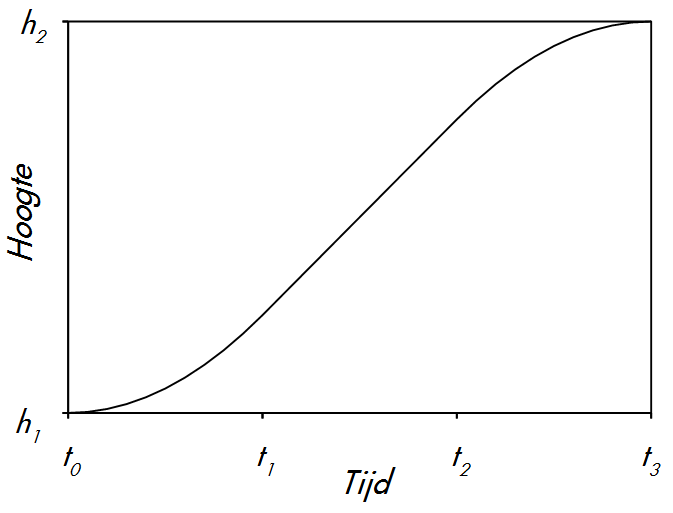
\includegraphics[width=0.31\linewidth]{HoogteRegeling/hoogte}}
\hspace{0.01\linewidth}
\subfigure[Snelheid]{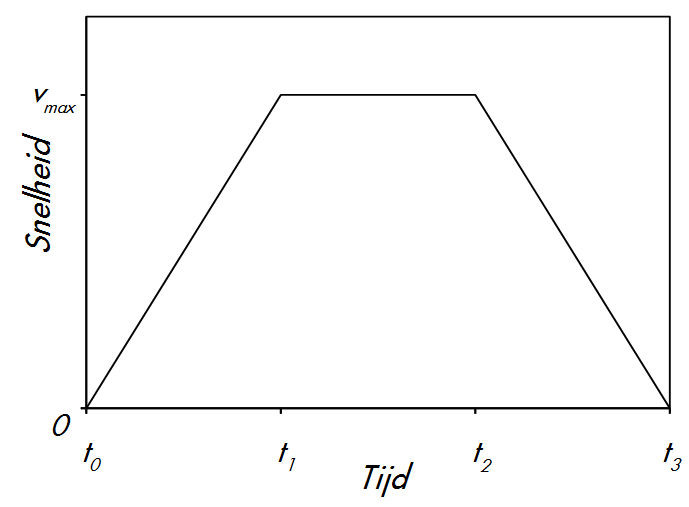
\includegraphics[width=0.31\linewidth]{HoogteRegeling/snelheid}}
\hspace{0.01\linewidth}
\subfigure[Versnelling]{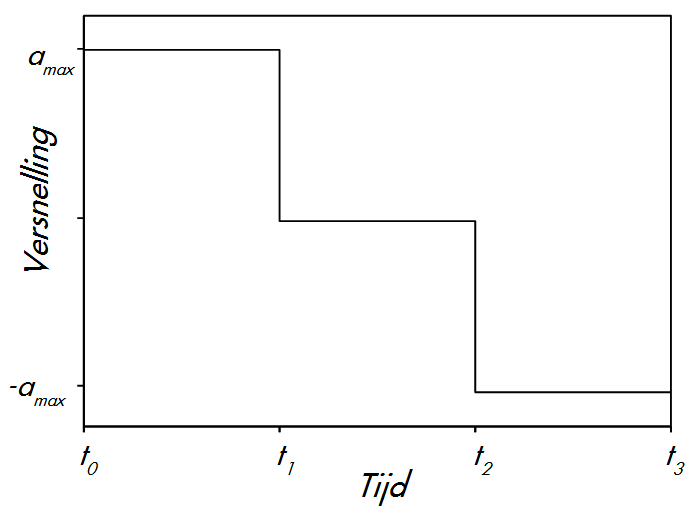
\includegraphics[width=0.31\linewidth]{HoogteRegeling/versnelling}}
\caption{Gewenst hoogte-, snelheids- en versnellingsprofiel}\label{fig:hsvprofiel}
\end{figure}

% referentie ERB
\noindent De profielen in figuur \ref{fig:hsvprofiel} kunnen voor iedere nieuwe setpoint berekend worden aan de hand van formules \eqref{eq:hoogtehoogtes} en \eqref{eq:hoogtetijden}. Deze formules zijn eenvoudig te vinden door de formules van de  \textit{\'e\'enparige rechtlijnige beweging} (ERB) om te vormen.

\begin{equation}
\left\{
\begin{matrix*}[l]

h(t) = h_1 + \frac{v_{max}^2}{2 \cdot a_{max}} \cdot t & \text{ als } t \leq t_1 \\
h(t) = h(t_1) + {v_{max}} \cdot t & \text{ als } t_1 < t \leq t_2 \\
h(t) = h(t_2) + \frac{v_{max}^2}{2 \cdot a_{max}} \cdot (t_2-t) & \text{ als } t_2 < t
\end{matrix*}
\right.
\label{eq:hoogtehoogtes}
\end{equation}

\begin{equation}
t_1 = \frac{v_{max}}{a_{max}},\ 
t_2 = (h_2-h_1)-\frac{v_{max}^{2}}{2 \cdot a_{max}}
\label{eq:hoogtetijden}
\end{equation}

\npar Bij implementatie van deze functiegenerator werd eerst een eenvoudigere versie geprogrammeerd. Deze eenvoudige versie beperkt enkel $v_{max}$. De gewenste hoogte neemt dan lineair toe met de tijd, tot de setpoint bereikt is. Uit de resultaten zal blijken dat deze eenvoudige aanpak ook volstaat.

\subsection{Optimalisatie PID parameters} \label{sec:optPID}
Na de optimalisaties in \ref{sec:autotakeoff} en \ref{sec:functiegen}, moet de hoogte regelaar ook eens bekeken worden. Om de ideale parameters te vinden, wordt gebruik gemaakt van de Ziegler-Nichols methode \cite{paper:ZieglerNichols}. De proportionele factor wordt opgedreven totdat de respons een oscillatie is met constante amplitude. De waarde voor de proportionele factor wordt de \textit{ultieme gain} genoemd. De ultieme gain wordt symbolisch voorgesteld als $K_u$. De oscillatieperiode wordt als $T_u$ voorgesteld. Volgens Ziegler-Nichols zijn de parameters die berekend kunnen worden met \eqref{eq:PIDpar} een goed uitgangspunt. 
\begin{equation}
	\centering
	P = 0.6 \cdot K_u,\ I = \dfrac{2 \cdot P}{T_u} \text{ en }D = \dfrac{K_p \cdot T_u}{8}
	\label{eq:PIDpar}
\end{equation}

\npar De met \eqref{eq:PIDpar} bekomen parameters zorgen nog voor zichtbare oscillaties. Bovendien is de responstijd vrij traag. De parameters moeten dus nog wat bijgeregeld worden. Om op een correcte manier te werk te gaan, wordt gesteund op het werk van K.\,H. Ang et al.\cite{paper:PIDtuning}. In deze paper wordt beschreven hoe een parameter moet aangepast worden om een bepaald effect te bekomen in het stapantwoord. Na een aantal tussenstappen wordt het gewenst gedrag bereikt. De proportionele- en differenti\"erende factor zijn nu wat hoger en de integrerende factor is verlaagd.

\subsection{Resultaat}
De optimalisatie van de drempelwaarde voor lift-off heeft vooral invloed op hoe snel het platform de gewenste hoogte bereikt net na het opstijgen. Als de lift-off waarde te laag gekozen wordt, dan is $Thr_0$ bijgevolg ook te laag. De integrerende factor moet dan de vaste fout op $Thr_0$ opvangen. Dit is te zien op figuur \ref{fig:opstijgen}(a). Wanneer de lift-off waarde wel goed gekozen wordt, zoals in figuur \ref{fig:opstijgen}(b), gaat het platform onmiddellijk naar de gewenste hoogte, weliswaar met een lichte overshoot.

\begin{figure}
	\begin{center}
		\subfigure[Lage lift-off drempelwaarde]{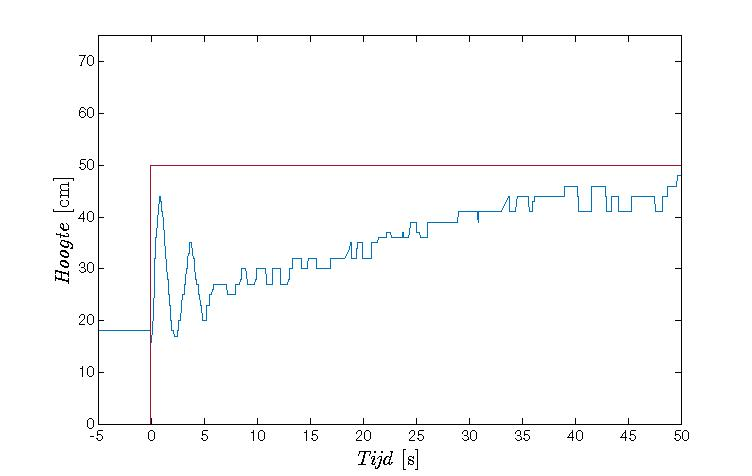
\includegraphics[width=0.8\linewidth]{HoogteRegeling/original}}
		
		\subfigure[Goede lift-off drempelwaarde]{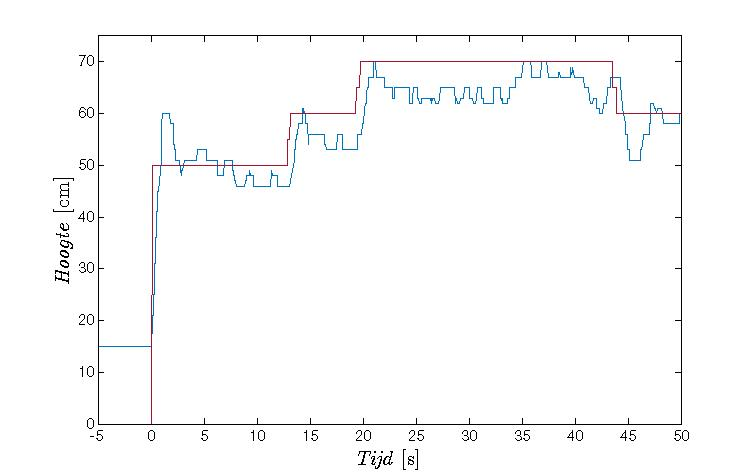
\includegraphics[width=0.8\linewidth]{HoogteRegeling/autotakeoff}}
	\end{center}
	\centering
	\caption{De invloed op het opstijggedrag van de quadcopter bij een te lage lift-off drempelwaarde in (a) en bij een goede lift-off drempelwaard in (b). Wanneer de drempelwaarde te laag gekozen is, duurt het een heel eind vooraleer de integrerende term van de PID-regelaar de vaste fout op $Thr_0$ heeft opgevangen.}\label{fig:opstijgen}
\end{figure}

\npar Overshoot is niet gewenst, dus die moet nog weggewerkt worden. Dit is de taak van de functiegenerator. Om de prestatie van de hoogte regeling zonder en met functiegenerator te vergelijken, wordt tijdens een testvlucht met de gewenste hoogte gespeeld. De reactie van het platform zonder en met functiegenerator wordt weergegeven in respectievelijk figuur \ref{fig:finaleHoogteRegeling}(a) en \ref{fig:finaleHoogteRegeling}(b). Het gebruik van een functiegenerator zorgt ervoor dat overshoot afneemt en dat de gewenste hoogte beter gevolgd wordt.

\begin{figure}
	\begin{center}
		\subfigure[Zonder functiegenerator]{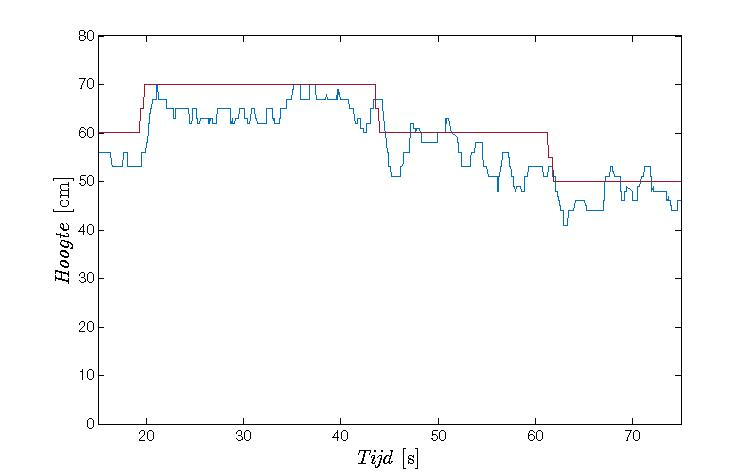
\includegraphics[width=0.8\linewidth]{HoogteRegeling/autotakeoffPID}}
		
		\subfigure[Met functiegenerator]{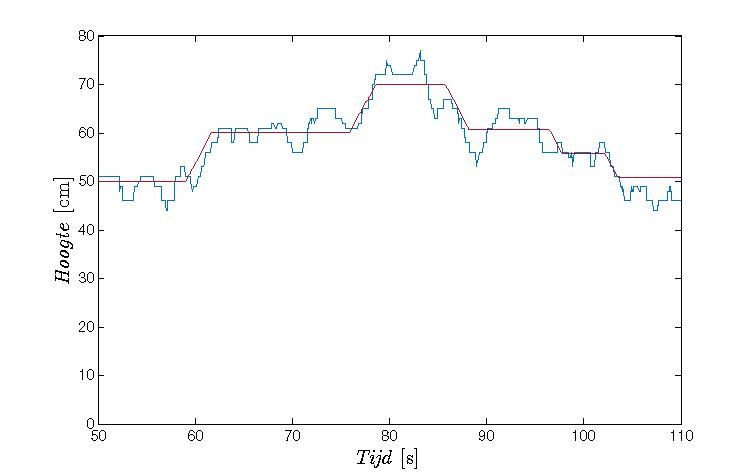
\includegraphics[width=0.8\linewidth]{HoogteRegeling/final}}
	\end{center}
	\centering
	\caption{Vergelijking tussen het vlieggedrag zonder en met functiegenerator. Wanneer de functiegenerator wordt aangezet, volgt de hoogte mooi de gewenste hoogte en is er minder overshoot dan wanneer de functiegenerator afligt.}\label{fig:finaleHoogteRegeling}
\end{figure}

\npar Er kan besloten worden dat het platform nu in staat is naar een bepaalde hoogte te navigeren zonder al te veel overshoot. De nieuwe hoogte regeling is in zijn opzet geslaagd. De optimalisatie van auto-land heeft weinig invloed op het vlieggedrag en wordt om die reden niet besproken bij de resultaten.


\section{Driftcompensatie}
In deze sectie wordt de driftcompensatie herzien. De drift van het platform wordt gemeten met behulp van optical flow. In \ref{sec:OptFlow} werd de werking van optical flow reeds uit de doeken gedaan. In sectie \ref{sec:OptFlowopt} werd de nauwkeurigheid van het algoritme verbeterd.

\npar Driftcompensatie op basis van optical flow is reeds aanwezig in de thesis van W. De Gucht, maar bij aanvang van deze thesis werkte dit helaas niet. Steunend op zijn werk wordt het opnieuw ingevoerd, met enkele aanpassingen weliswaar. Driftcompensatie kan gesplitst worden in twee delen. Op de eerste plaats moet de positie van het platform gemeten kunnen worden ten opzichte van de vorige positie. Pas dan kan drift gedetecteerd worden. Ten tweede is er de compensatie zelf. Van zodra drift gedetecteerd wordt, moet die gecompenseerd worden.

\subsection{Drift detecteren}
Het pijnpunt van de oorspronkelijke driftdetectie is dat er verondersteld wordt dat nieuwe optical flow data altijd met \SI{20}{\Hz} binnenkomt. Dit is in de praktijk echter niet het geval, er zit wat variatie op. Bijgevolg klopt de compensatie van de flow vectoren met roll en pitch niet volledig. Om dezelfde reden zijn de integratieterm en de differentiatieterm van de PID-regelaar ook niet correct. Door gewoon het tijdsverschil tussen de twee frames waarover optical flow berekend wordt mee te geven, kunnen deze twee problemen in \'e\'en keer worden opgelost.

\npar Er blijft echter wel nog steeds een probleem over bij de compensatie van de flow vectoren met roll en pitch. Door het verleggen van de optical flow berekeningen naar de PC, zit er een extra vertraging op de optical flow vectoren. Dit betekent dat de compensatie met roll en pitch verschoven moet worden. In \ref{sec:resultaatVerleggen} werd reeds vermeld dat de vertraging drie tijdstappen bedraagt.

\subsection{Drift compenseren}
Na het detecteren van drift moet er uiteraard ook compensatie volgen. Hiervoor moet de positie regelaar herzien worden. Deze wordt een stuk vereenvoudigd. Er wordt enkel nog gebruik gemaakt van een PI-regelaar die de snelheid regelt. De quadcopter kan dan in positie gehouden worden door zijn snelheid op nul te regelen.

\npar Om van positie te veranderen, wordt het wel iets ingewikkelder. Er moet gedurende een bepaalde tijd een gewenste snelheid opgelegd worden in de juiste richting. Deze snelheid moet dan weer naar nul gezet worden eens de positie bereikt is. In principe is dit volledig analoog aan hetgeen in \ref{sec:functiegen} werd toegepast. De positie zal lineair vari\"eren in functie van de tijd.

\subsection{Resultaten}
De nieuwe manier voor het compenseren van drift kan niet getest worden. Het platform reageert niet op de controlesignalen die worden aangelegd om pitch en roll te veranderen. Er wordt vermoed dat dit te wijten is aan het ontbreken van een afstandbediening. Normaal wordt de afstandbediening gebruikt voor het aanleggen van het gewenste vlieggedrag. Wanneer de afstandsbediening ontbreekt worden de variabelen die dit gedrag bijhouden niet correct ge\"initialiseerd. Bijgevolg is het niet mogelijk om het gewenst gedrag aan te passen.

\section{APM logica}
Naast het invoeren van optimalisaties moest ook heel wat code herschreven worden. Bij de code van W. De Gucht steunt de status van het platform voor een groot stuk op de signalen die gegeven worden door zijn afstandsbediening. Voor deze thesis was geen afstandbediening beschikbaar. Bovendien zijn een aantal statussen van het platform overbodig geworden, juist omdat er geen afstandsbediening meer gebruikt wordt. De nieuwe APM logica wordt afgebeeld in figuur \ref{fig:APMlogic}.

\begin{table}[h]
	\caption{Nieuwe commando's om het vlieggedrag te be\"invloeden.}\label{table:newcom}
	\centering
	\begin{tabular}{cp{.7\linewidth}}
		\cr
		\hline
		Commando & Betekenis \\
		\hline
		i & Auto-takeoff, de quadcopter laat zijn throttle stijgen tot lift-off wordt gedetecteerd. \\
		u & Auto-land, de quadcopter gaat langzaam dalen. \\
		y & Leg optical flow aan of uit.\\
		\hline	
	\end{tabular}
\end{table}


\npar De lijst met commando's die de RPi kan geven, is met drie commando's uitgebreid. Hun betekenis wordt nog eens opgelijst in tabel \ref{table:newcom}. Pas als optical flow wordt geactiveerd, kan een vaste positie aangehouden worden. Het is niet aangeraden om optical flow te activeren tijdens het opstijgen, zie \ref{sec:hoogtereg}.

\section{Besluit}
In dit hoofdstuk werden een aantal optimalisaties voorgesteld. Helaas werkt de driftcompensatie nog niet. Hoewel dit in theorie zou moeten werken is dit in praktijk niet het geval door het ontbreken van de afstandsbediening. Dit heeft belangrijke gevolgen voor de komende hoofdstukken over omgevingsmapping. De testen voor het mappen zullen steeds moeten gebeuren met de quadcopter in de hand.

\begin{figure}[h]
	\centering
	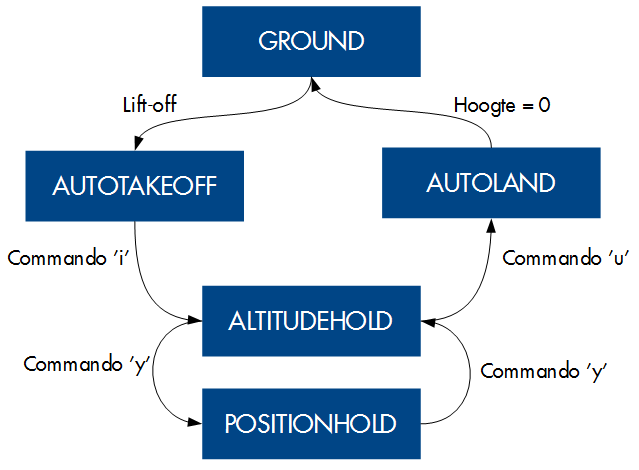
\includegraphics[width=0.7\linewidth]{APMlogic}
	\caption{Logica op de APM. De statussen worden afgebeeld in de rechthoeken. De condities voor een transitie worden afgebeeld naast de pijlen.} \label{fig:APMlogic}
\end{figure}



